\documentclass{standalone}
\usepackage{tikz}
\usepackage{setspace}
\usepackage{pgfplots}
\pgfplotsset{compat=1.15}
\pgfplotsset{soldot/.style={only marks,mark=*, line width=0.2pt, mark size=1.5pt}}
\pgfplotsset{holdot/.style={fill=white,only marks,mark=*, line width=1.0pt, mark size=1.5pt}}

\begin{document}
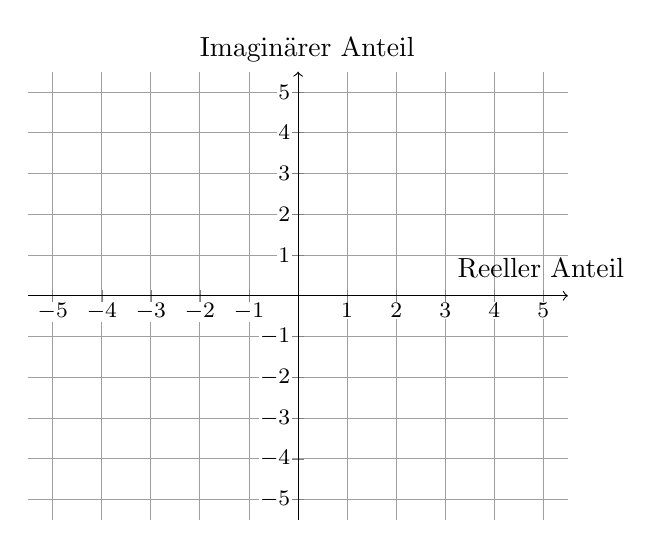
\begin{tikzpicture}
    \begin{axis}[
      grid=both, 
      grid style={line width=0.35pt, draw=gray!75},
      axis lines=center,
      axis line style={black,->},
      x label style={at={(axis description cs:0.95,0.52)},anchor=south},
      y label style={at={(axis description cs:0.3,1.05)},anchor=west},
      xlabel={Reeller Anteil},
      ylabel={Imaginärer Anteil},
      xmin=-5.5, xmax=5.5,
      ymin=-5.5, ymax=5.5,
      xtick={-5,-4,...,5},
      ytick={-5,-4,...,5},
      ticklabel style={font=\footnotesize,inner sep=0.5pt,fill=white,opacity=1.0, text opacity=1},
      every axis plot/.append style={line width=1.5pt, color=black},
      ]
        %% Using 'samples at' instead of domain to control plotting discontinuities
      \end{axis}
    \end{tikzpicture}
\end{document}
